\documentclass[10pt,twocolumn]{article}

% Pacchetti di base
\usepackage[utf8]{inputenc}
\usepackage{geometry}
\geometry{a4paper, left=1.5cm, right=1.5cm, top=2cm, bottom=2cm}

% Pacchetti aggiuntivi
\usepackage{graphicx} 
\usepackage{hyperref} % Per collegamenti ipertestuali
\usepackage{titlesec} % Per personalizzare i titoli
\usepackage{abstract} % Per formattare l'abstract
\usepackage{cite} 

\usepackage{url}

\usepackage{dsfont}
\usepackage{booktabs}
\usepackage{amsmath}
\usepackage{amssymb}
\usepackage{wrapfig} % Include this line in your preamble
\usepackage{float}

% Impostazioni dei titoli delle sezioni
\titleformat{\section}{\Large\bfseries}{\thesection.}{1em}{}
\titleformat{\subsection}{\large\bfseries}{\thesubsection.}{1em}{}

% Intestazione e piede di pagina
\usepackage{fancyhdr}
\pagestyle{fancy}
\fancyhf{}
\fancyhead[C]{Multiple instance learning with pre-contextual knowledge - Andrea Grandi, Daniele Vellani}
\fancyfoot[C]{\thepage}

% Dati del documento
\title{\textbf{Multiple instance learning with pre-contextual knowledge}}
\author{Andrea Grandi, Daniele Vellani \\
\texttt{\{275074,196186\}@studenti.unimore.it}}
\date{Data}

\begin{document}

% Titolo e Autore
\maketitle

% Abstract
\begin{abstract}
\noindent 
The visual examination of histopathological images is a cornerstone of cancer diagnosis, requiring pathologists to analyze tissue sections across multiple magnifications to identify tumor cells and subtypes. However, existing attention-based Multiple Instance Learning (MIL) models for Whole Slide Image (WSI) analysis often neglect contextual and numerical features, resulting in limited interpretability and potential misclassifications. Furthermore, the original MIL formulation incorrectly assumes the patches of the same image to be independent, leading to a loss of spatial context as information flows through the network. Incorporating contextual knowledge into predictions is particularly important given the inclination for cancerous cells to form clusters and the presence of spatial indicators for tumors. To address these limitations, we propose an enhanced MIL framework that integrates pre-contextual numerical information derived from semantic segmentation. Specifically, our approach combines visual features with nuclei-level numerical attributes, such as cell density and morphological diversity, extracted using advanced segmentation tools like Cellpose. These enriched features are then fed into a modified BufferMIL model for WSI classification. We evaluate our method on subtyping non-small cell lung cancer (TCGA-NSCLC) and detecting lymph node metastases (CAMELYON16 and CAMELYON17).

\end{abstract}

\section{Introduction}
In recent years, computational pathology has emerged as a transformative tool for cancer research, leveraging Whole Slide Images (WSIs) to extract meaningful insights into tissue architecture and cellular composition. These large, high-resolution images are invaluable for diagnosing and prognosticating cancer, yet their sheer size, heterogeneity, and reliance on detailed annotations pose substantial challenges. One computational challenge is the large size of WSIs, of the order of 100,000 $\times$ 100,000 pixels. Processing images of such size with deep neural network directly is not possible with the GPUs commonly available. Overcoming this problem, previous work proposes to tessellate each WSI into thousands of smaller images called tiles and global survival prediction per slide is obtained in two steps. The tiles are first embedded into a space of lower dimension using a pre-trained feature extractor model, and a MIL model is trained to predict survival from the set of tiles embeddings of a WSI (Herrera et al., 2016)\cite{8507932}. 

Multiple Instance Learning (MIL) has become a pivotal paradigm for WSI analysis. By treating a slide as a "bag" of smaller patches (instances), MIL allows slide-level predictions without the need for pixel-level annotations, streamlining the analysis pipeline (Ilse et al., 2018; Campanella et al., 2019)\cite{ilse2018attention, campanella2019clinical}. Despite its utility, traditional MIL approaches often overlook critical contextual and numerical information that can enhance interpretability and predictive accuracy.

One limitation of MIL is the assumption that tiles from the same WSI are independent (Ilse et al., 2018)\cite{ilse2018attention}. In particular, MIL models take into account only the visual knowledge comes from WSIs. In contrast, pathologists take into account also other aspects of WSIs in their analysis. Addressing these limitations requires innovative approaches capable of combining visual and numerical features from WSIs effectively (Litjens et al., 2017; Campanella et al., 2019) \cite{litjens2017survey, campanella2019clinical}.

In this work, we introduce a novel pipeline that integrates cutting-edge tools and methodologies to overcome these limitations. We preprocess WSIs using the CLAM framework (Lu et al., 2021) \cite{lu2021clam}, ensuring the retention of essential visual features. To extract nuclei-specific numerical features such as cell counts and density, we utilize Cellpose (Stringer et al., 2021) \cite{stringer2021cellpose}, a state-of-the-art segmentation algorithm. Simultaneously, we employ DINO (Caron et al., 2021) \cite{caron2021emerging}, a self-supervised vision transformer, to generate embeddings representing the visual content of each patch. By concatenating these numerical and visual features, we construct a richer, more informative representation for each patch.

Our key innovation lies in adapting the BufferMIL (Bontempo et al, 2023)\cite{10.1007/978-3-031-43153-1_1} framework to incorporate these enriched embeddings, enhancing interpretability through the extracted numerical features.

%By assigning greater importance to patches with high cell density or other critical numerical features, our model improves sensitivity to diagnostically relevant regions. This dual-feature approach enhances both interpretability and predictive performance, addressing long-standing challenges in WSI classification.

This paper is structured as follows: Section \ref{related} reviews key advancements in MIL and its applications in computational pathology. Section \ref{methods} describes our methodology, detailing preprocessing, feature extraction, and the enhancements made to BufferMIL. Section \ref{results} presents experimental results, discusses their implications, and outlines potential future directions. By combining numerical and visual features, our work seeks to advance computational pathology and provide deeper insights into the analysis of WSIs.

The source code is publicly available at \url{https://github.com/andrea-grandi/bio_project}.

\section{Related Work} \label{related}
Multiple Instance Learning has revolutionized computational pathology by enabling efficient WSI classification without exhaustive pixel-level annotations. Under MIL formulation, the prediction of a WSI label can come either directly from the tile predictions (instance-based) (Campanella et al.,2019)\cite{campanella2019clinical}, or from a higher-level bag representation resulting from aggregation of the tile features (bag embedding-based) (Ilse et al., 2018)\cite{ilse2018attention}. The bag embedding-based approach has empirically demonstrated superior performance (Sharma et al., 2021)\cite{conf/midl/SharmaSEMSB21}. Most recent bag embedding-based approaches employ attention mechanisms, which assign an attention score to every tile reflecting its relative contribution to the collective WSI-level representation. Attention scores enable the automatic localization of sub-regions of high diagnostic value in addition to informing the WSI level label.

One of the first important work in this field was DS-MIL (Li et al., 2021)\cite{li2021dualstreammultipleinstancelearning}. This model utilizes a dual-stream framework, where patches are extracted from different magnifications (e.g., 5× and 20× in their study) of Whole Slide Images. These patches are processed separately for self-supervised contrastive learning. The embeddings obtained from patches at various resolutions are then concatenated to train the MIL aggregator, which assigns an importance or criticality score to each patch. The most critical patch is selected and compared to all others in a one-vs-all manner. This comparison uses a distance metric inspired by attention mechanisms, though it differs significantly by comparing two queries instead of the traditional key-query setup. Finally, the distances are aggregated to generate the final bag-level prediction.

Another work is BufferMIL, which is a notable framework that enhances MIL by incorporating explicit domain knowledge for histopathological image analysis, particularly addressing challenges like class imbalance and covariate shift. In this approach, a buffer is maintained to store the most representative instances from each disease-positive slide in the training set. An attention mechanism then compares all instances against this buffer to identify the most critical ones within a given slide. This strategy ensures that the model focuses on the most informative instances, thereby improving its generalization performance. By leveraging a buffer to track critical instances and employing an attention mechanism for comparison, Buffer-MIL effectively mitigates issues related to class imbalance and covariate shift. This approach enhances the model's ability to focus on the most informative patches within WSIs, leading to more accurate and reliable predictions in histopathological image analysis.

Building upon the attention-based methodologies of frameworks like BufferMIL, Context-Aware MIL (CAMIL) (Fourkioti et al., 2024)\cite{fourkioti2023camil} extends the concept of informed instance selection by introducing neighbor-constrained attention mechanisms. CAMIL leverages spatial dependencies among WSI tiles to achieve superior performance in cancer subtyping and metastasis detection, showcasing the importance of spatial context in WSI analysis. Similarly, the Nuclei-Level Prior Knowledge Constrained MIL (NPKC-MIL) (Wang et al., 2024)\cite{WANG2024109826} highlights the value of combining handcrafted nuclei-level features with deep learning, demonstrating improvements in interpretability and classification accuracy for breast cancer WSIs.

%Building on these advancements, our approach integrates nuclei-specific numerical features extracted via Cellpose into the BufferMIL framework. This integration enriches the bag representation with critical cellular attributes, such as density and morphological diversity, while leveraging high-dimensional visual embeddings from DINO. This combination bridges the gap between domain-specific insights and generalizable deep learning models, pushing the boundaries of WSI analysis.

%In summary, the integration of prior knowledge into MIL frameworks, exemplified by BufferMIL, CAMIL, and NPKC-MIL, represents a paradigm shift. These models enhance both classification performance and interpretability, offering promising tools for computational pathology and personalized medicine.

\begin{figure}[!htb]
\centering
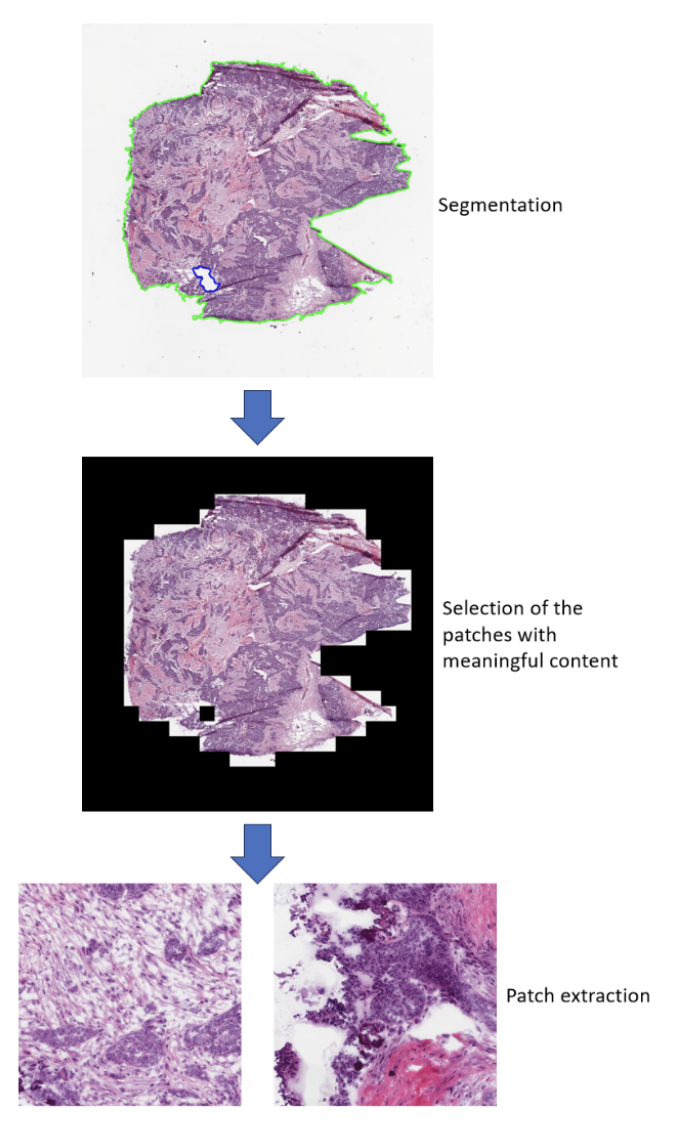
\includegraphics[width=0.4\textwidth, height=12cm]{images/wsi_preprocess.png}
\caption{Whole Slide Image Preprocessing} 
\label{wsi_preprocessing}
\end{figure}

\section{Methods} \label{methods}

In this section, we detail the methodology employed in our study, focusing on the integration of numerical and visual features into an enhanced MIL framework for WSI analysis.

\begin{figure*}[!htb]
\centering
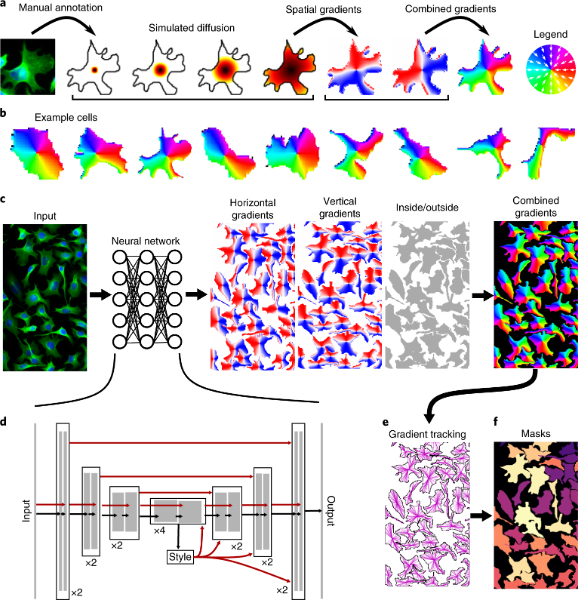
\includegraphics[width=0.65\textwidth, height=8cm]{images/cellpose.png}
\caption{\textbf{Model architecture. a}, Procedure for transforming manually annotated masks into a vector flow representation that can be predicted
by a neural network. A simulated diffusion process started at the center of the mask is used to derive spatial gradients that point towards the
center of the cell, potentially indirectly around corners. The X and Y gradients are combined into a single normalized direction from 0 to 360.
\textbf{b}, Example spatial flows for cells from the training dataset. \textbf{cd}, A neural network is trained to predict the horizontal and vertical flows, as well
as whether a pixel belongs to any cell. The three predicted maps are combined into a flow field. \textbf{d} shows the details of the neural network
which contains a standard backbone neural network that downsamples and then upsamples the feature maps, contains skip connections
between layers of the same size, and global skip connections from the image styles, computed at the lowest resolution, to all the successive
computations. \textbf{e}, At test time, the predicted flow fields are used to construct a dynamical system with fixed points whose basins of attraction
represent the predicted masks. Informally, every pixel ”follows the flows” along the predicted flow fields towards their eventual fixed point. \textbf{f}, All
the pixels that converge to the same fixed point are assigned to the same mask.} 
\label{cellpose}
\end{figure*}


\subsection{Patch Extraction and Preprocessing}

In our study, we employed the CLAM (Computational Pathology Learning and Analysis Methods) framework to efficiently extract patches from Whole Slide Images (WSIs) at a magnification of 20x. This magnification was chosen for its balance between detail and computational manageability, providing sufficient resolution for histopathological analysis. The extraction process involved several key steps as shown in Figure \ref{wsi_preprocessing}:

\begin{itemize}
    \item \textbf{Patch Extraction with CLAM}: CLAM was used to divide the large WSIs into smaller, manageable patches. This framework is designed to handle the scale and complexity of WSIs by extracting patches at specified magnifications, in this case, 20x.

    \item \textbf{Otsu's Thresholding}: To segment the tissue areas from non-tissue regions within each patch, we applied Otsu's thresholding method. Otsu's algorithm automatically determines the optimal threshold value to separate the foreground (tissue) from the background, based on the image's histogram. This step is crucial for focusing the analysis on relevant tissue regions and reducing noise from non-tissue areas.
   

    \item \textbf{Storage in .h5 Format}: The thresholded patches were stored in .h5 format by CLAM. This format is efficient for storing large datasets and includes the processed images along with any associated metadata.

    \item \textbf{Conversion to .jpg Format}: For compatibility with standard image processing pipelines and ease of use in downstream processing, we converted the .h5 files to .jpg format. This conversion ensures that the patches can be easily integrated into various image processing libraries and neural network models.
\end{itemize}

The choice of Otsu's thresholding was motivated by its effectiveness in segmenting histopathological images, while CLAM was selected for its efficiency in handling large WSIs and extracting patches at different magnifications. The conversion to .jpg format was necessary to maintain compatibility with widely used image processing tools, with minimal impact on the quality of the patches for feature extraction.


\subsection{Feature Extraction}

Our approach involves the extraction of both visual and numerical features from the patches.

\subsubsection{Visual Feature Extraction with DINO}

%We utilized DINO (Data-Independent Neighborhood Occupancy) \cite{caron2021emerging}, a self-supervised vision transformer, to extract high-dimensional visual embeddings from the patches. 
We utilize DINO (Data-Independent Neighborhood Occupancy) for visual embeddings because is particularly suited for this task due to its ability to capture rich visual information without requiring labeled data. The architecture of DINO is based on the ViT (Vision Transformer) (Dosovitskiy et al., 2021) \cite{dosovitskiy2021imageworth16x16words}, which processes images by dividing them into patches and passing them through a series of transformer encoder layers. 

DINO enhances the self-supervised learning process by introducing teacher and student networks, where the teacher network provides pseudo-labels for the student network. This approach allows the model to learn robust representations by minimizing the distance between the predictions of the student and teacher networks. 

To extract the visual embeddings, we first preprocessed the image patches by resizing them to a fixed resolution compatible with the DINO model. We then fed these patches into the pre-trained DINO model to obtain the embeddings from a specific layer, which were used as the primary input for our MIL model. These embeddings capture the intricate visual details within each patch, providing a robust representation for subsequent analysis.



\subsubsection{Numerical Feature Extraction with Cellpose}

To incorporate numerical features, we employed Cellpose to extract nuclei-level attributes from the patches. Cellpose is designed to segment cyto and nuclei in histopathological images with high accuracy, enabling the computation of numerical features such as cell density and morphological diversity.

As we can see in Figure \ref{cellpose}, the segmentation process involves several steps. First, the image patches are preprocessed to enhance contrast and remove noise. Cellpose then applies a U-Net architecture (Ronneberger et al., 2015)\cite{ronneberger2015unetconvolutionalnetworksbiomedical} to predict cell boundaries and nuclei centers. Additionally, Cellpose predicts flow vectors, which are crucial for accurately segmenting overlapping or touching cells. These flow vectors represent the direction and magnitude from cell centers to the edges, aiding in the precise identification of individual cells.

From these predictions, we extracted numerical features including cell density (number of cells per unit area), average nucleus area, and morphological diversity (measured using shape descriptors such as circularity and eccentricity). To further enhance the feature set, we derived features from the flow vectors, such as the mean and variance of flow directions and magnitudes within each patch. These flow-based features provide additional context about the cellular arrangement and organization.

We concatenated these numerical features with the visual embeddings from DINO to create a comprehensive representation of each patch, enhancing the discriminative power of our model. To ensure effective integration, we normalized the features, allowing them to contribute equally to the model's performance.

In summary, Cellpose not only segments cells but also provides flow vector information, which we leveraged to extract additional numerical features. This combined approach offers a more holistic representation of the cellular composition within each patch, complementing the visual information extracted from the images.

\subsubsection{Geometry Dataset Conversion}

To integrate the extracted features into the BufferMIL framework, we converted the data into a geometry dataset format, specifically into a DataBatch structure. This conversion is essential for ensuring compatibility with the input requirements of BufferMIL, which expects data in a specific format that includes both visual and numerical features.

The DataBatch structure organizes the data into batches, where each batch contains the concatenated features of multiple patches. We preprocessed the features by normalizing the numerical attributes to have zero mean and unit variance, ensuring that they are on a similar scale to the visual embeddings. We also ensured that the data is appropriately shuffled and split into training, validation, and test sets.

%This conversion process involved writing custom scripts to read the extracted features, perform the necessary preprocessing, and organize the data into the required format. By doing so, we enabled the BufferMIL model to effectively process the combined visual and numerical features, leveraging both types of information for improved classification performance.

%\begin{figure*}[!htb]
%\centering
%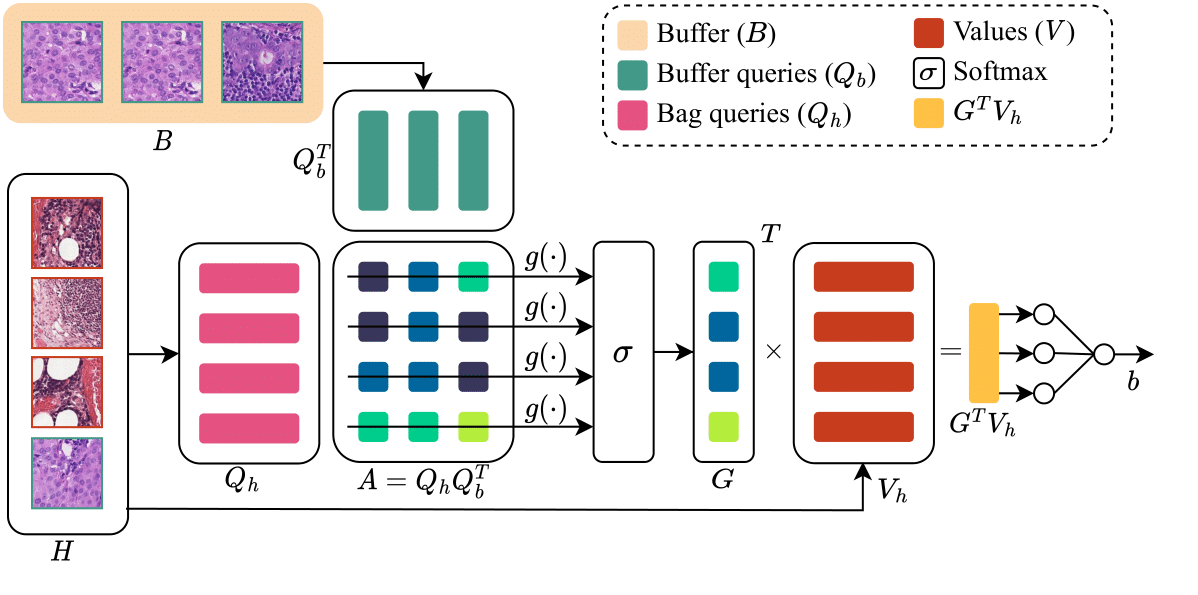
\includegraphics[width=0.8\textwidth, height=8cm]{images/buffermil.png}
%\caption{BufferMIL architecture} 
%\label{buffermil}
%\end{figure*}

\subsection{BufferMIL Adaptation}

To adapt BufferMIL, particularly the buffer selection of critical patches, we have implemented an embedding concatenation approach before incorporating them into the adjacency matrix. 

\subsubsection{Attention Mechanism}

The attention mechanism in BufferMIL is adapted to consider both structural and morphological features of patches. Given an adjacency matrix $A$ extracted from the higher-level representation, we normalize it using min-max scaling:

\begin{equation}
A = \frac{A - \min(A)}{\max(A) - \min(A)}
\end{equation}

Additionally, we normalize supplementary extracted features, such as the number of cells per patch, cell density, and mean cell area:


The computed scores are then stored in the buffer for selecting the top $n$ critical patches, refining the selection process and enhancing the robustness of the model.

\section{Experiments and Results} \label{results}

\section{Conclusions} \label{conclusions}

\bibliographystyle{unsrt}
\bibliography{references}

\end{document}